
\chapter{Test de performance}

Ce chapitre regroupe les tests qui ont été conduits afin d'essayer de quantifier les performances pouvant être atteintes par le système.

\section{Test de distance}

Ce test tente d'évaluer la distance maximale de fonctionnement de la communication LoRa du capteur. La portée de la communication étant un aspect important du système, une course test amenant une distance maximum d'un peu plus de 1 km entre le capteur et la passerelle est effectuée pour essayer de déterminer ce paramètre.

Le lieu choisi se trouve près de l'aérodrome de Colombier, le long de l'autoroute. Ce chemin offre un dégagement optimal afin de s'assurer d'avoir le moins d'obstacles possible.

La première tentative du test, effectué le 24 Septembre 2018, n'a pas été très concluante. Même si un paquet a été reçu depuis une distance d'environ 670 m, la plupart des paquets n'ont pas été reçus par la passerelle comme espéré. Néanmoins, ce test n'a pas été inutile, il a permis de déterminer que la puissance du signal avec la configuration de base ne permet pas d'atteindre des distances de plus de \todo{xxx m} avec un taux de perte de paquet qui soit satisfaisant. Il a donc été décidé de rééditer l'opération mais cette fois avec une valeur de puissance du signal plus haute. On notera que la puissance configurée pour le premier test était de -0.6 dBm avec un facteur d'étalement maximal de sf12.

On peut voir sur la figure \ref{fig:test_distance_11} les points qui ont été acquis durant la première édition du test de distance. Le point bleu symbolise la position de la passerelle.

\begin{figure}[htb]
\centering 
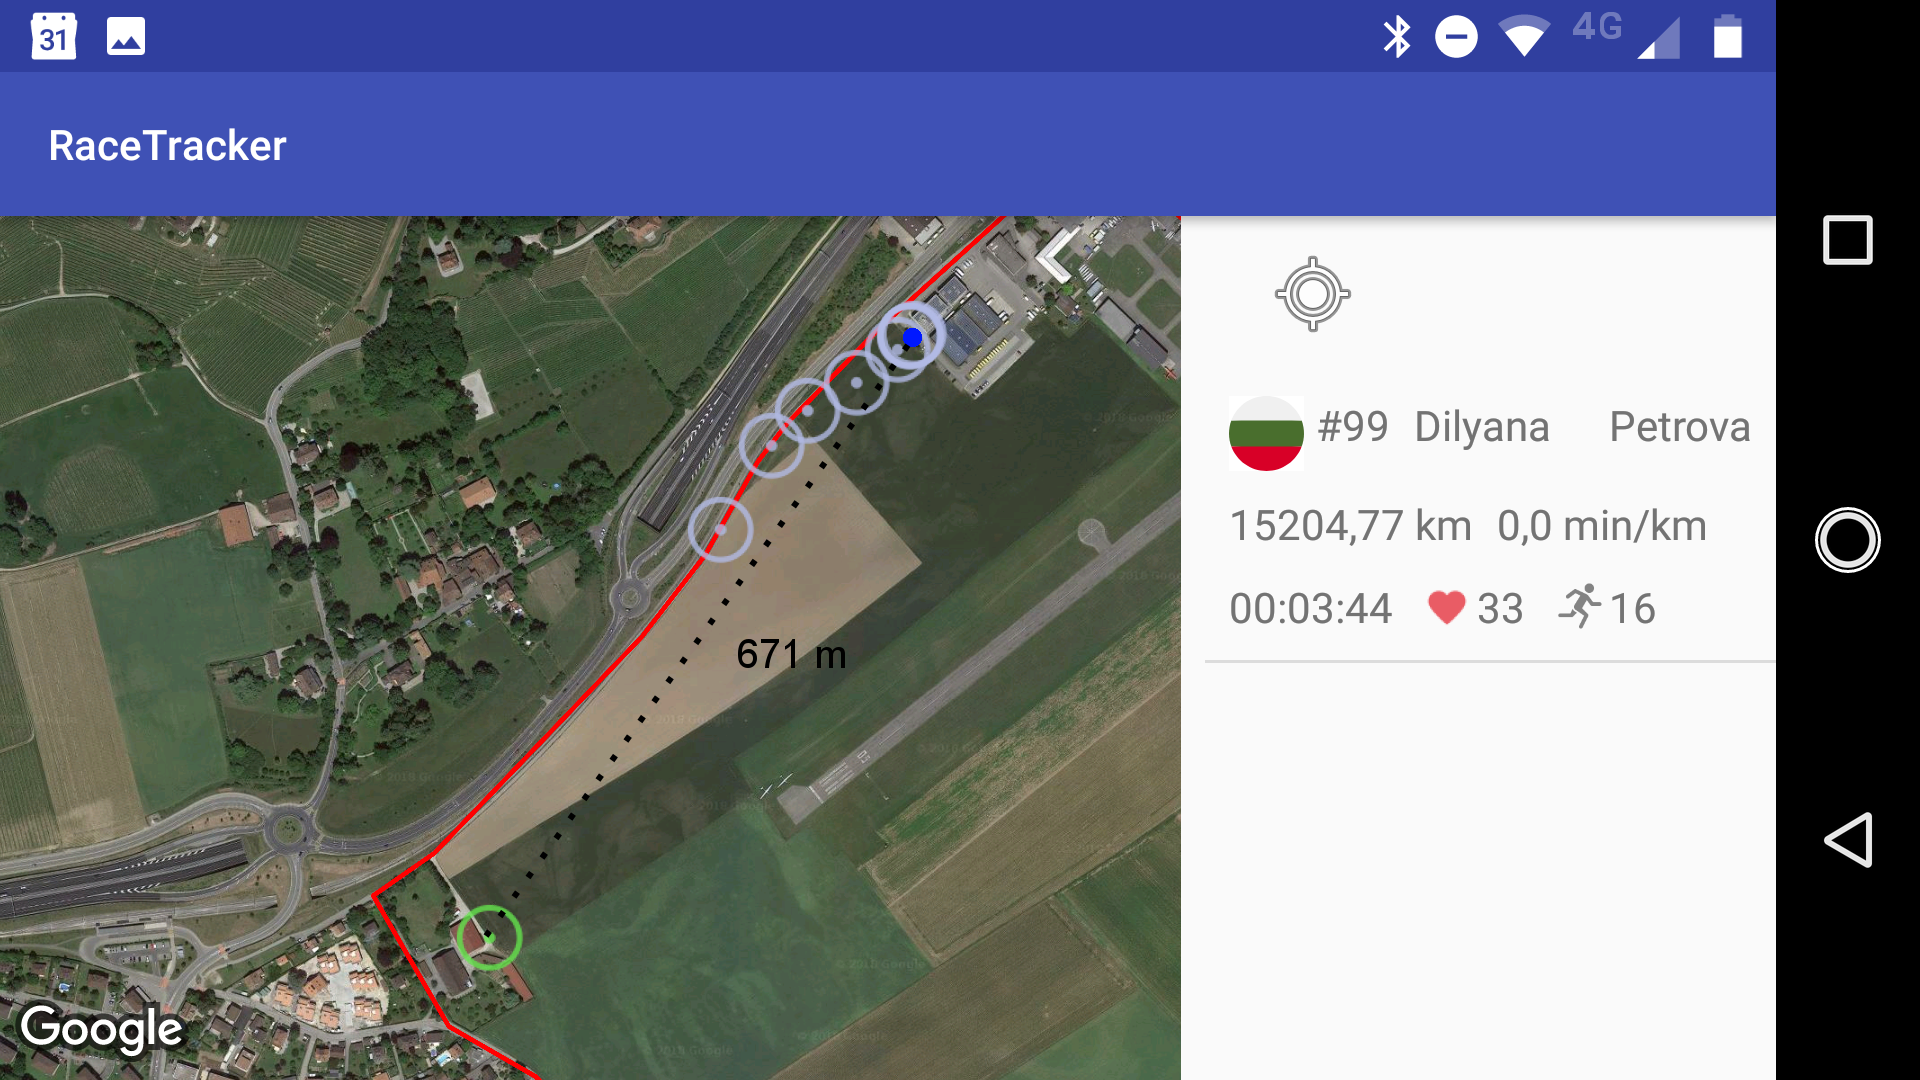
\includegraphics[width=0.9\columnwidth]{test_distance_1.png} 
\caption{Vue d'ensemble des positions récoltées durant le premier test}
\label{fig:test_distance_11}
\end{figure}

Une deuxième tentative a été réalisée le 25 Septembre 2018 au même endroit afin de pouvoir comparer les deux résultats. Cette fois-ci le capteur est configuré afin de délivrer une puissance au signal de sortie de 13.5 dBm et un facteur d'étalement similaire au premier test de sf12.

Sur la figure \ref{fig:test_distance_2_1} on peut voir la distance maximale atteinte durant le deuxième test ainsi que tous les points qui ont été acquis durant l'exercice. On remarque que les points sont reçus avec précision tout au long du parcours. Le point bleu montre la position de la passerelle pendant le test.

\begin{figure}[htb]
\centering
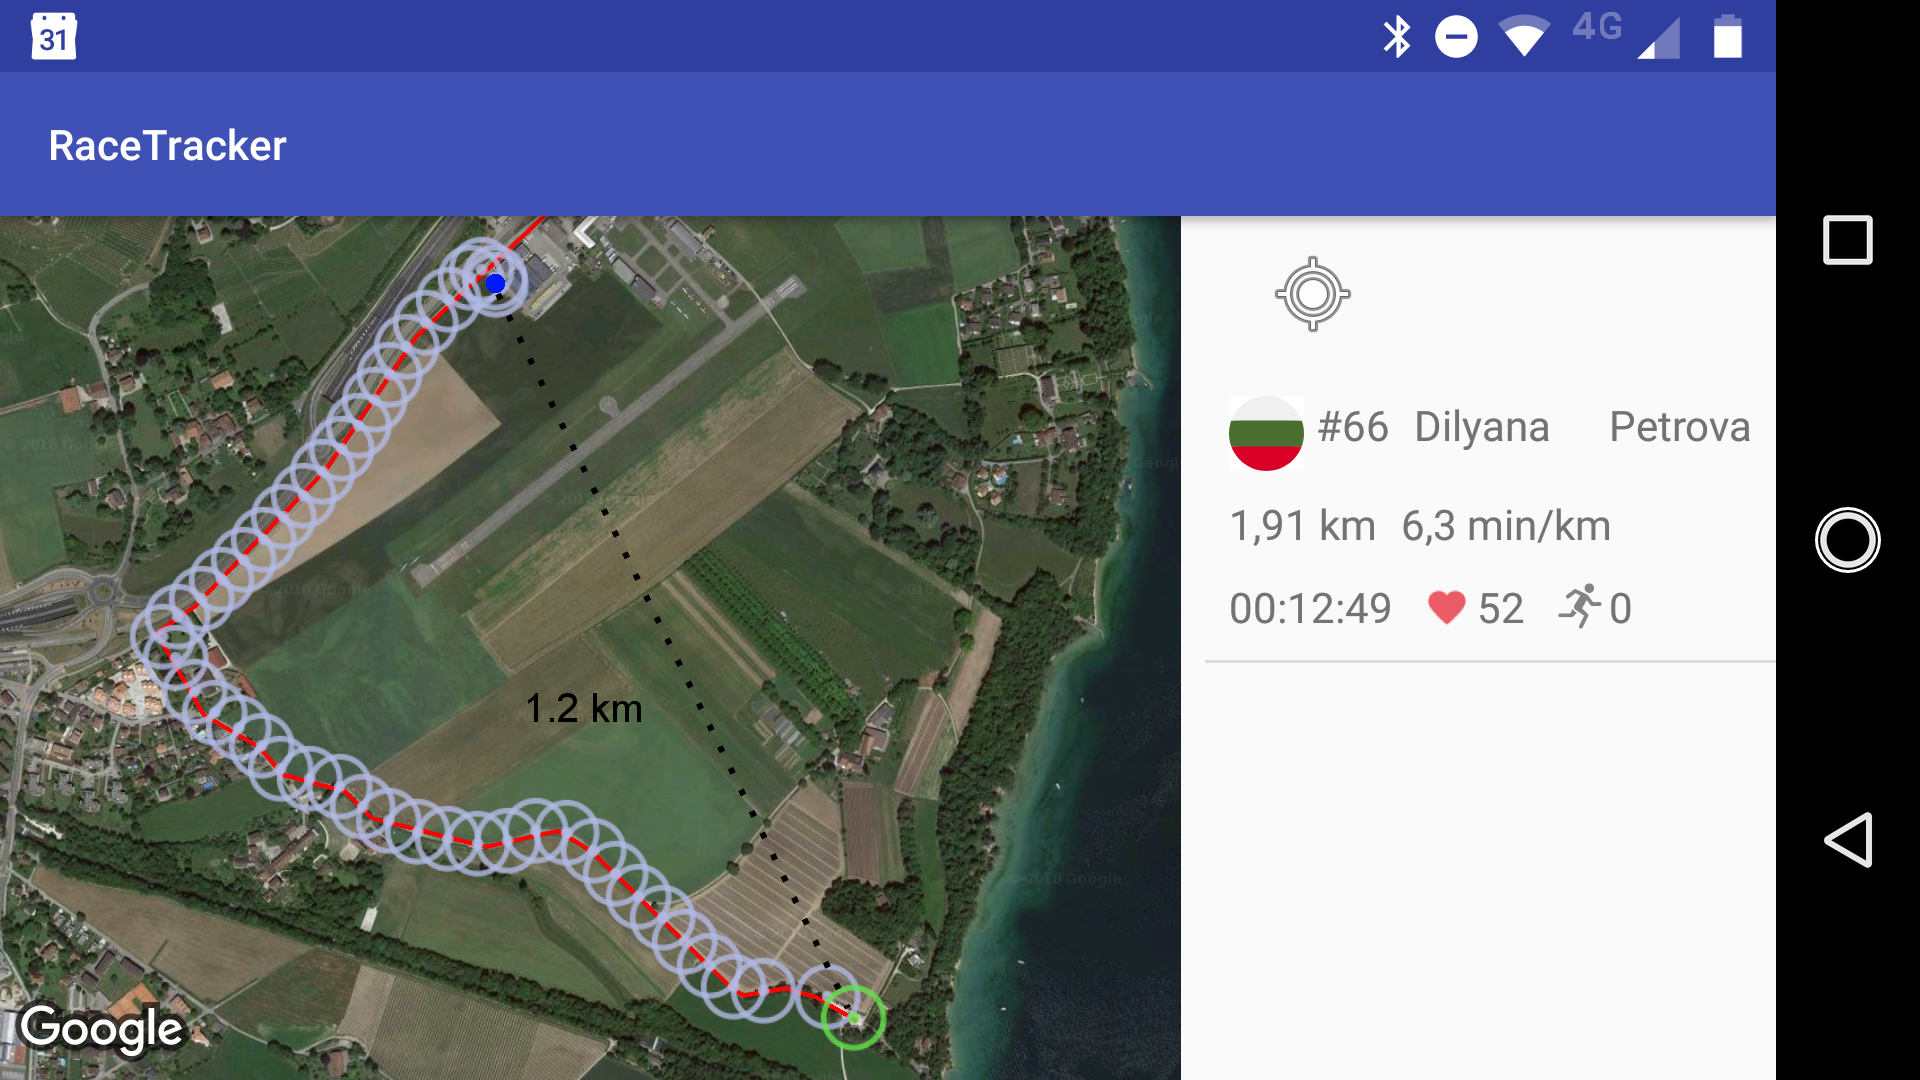
\includegraphics[width=0.9\columnwidth]{test_distance_2_1.png} 
\caption{Vue d'ensemble des positions récoltées durant le deuxième test}
\label{fig:test_distance_2_1}
\end{figure}

Sur la figure \ref{fig:test_distance_2_2} on peut voir le détail du parcours de la deuxième tentative du test de distance. On remarque que les points sont bien réguliers et qu'il n'y a pas de perte de paquet. On peut également constater que durant quelques mètres la vue entre la passerelle et le capteur a été totalement obstruée et les paquets ont quand même bien été reçus par la passerelle. Cela montre que contrairement à ce qui avait pu être constaté durant le test d'obstruction de la vue, voir chapitre \ref{ch:test_obstru}, si la puissance du signal est suffisante, les paquets peuvent quand même être reçus malgré le fait que la ligne de vue entre le capteur et la passerelle soit bouchée.

Ce test a permis de démontrer l'importance de la configuration de la puissance du signal. Lors de la première tentative, pratiquement aucun paquet n'a été reçu au-delà de quelques centaines de mètres, alors que pour la deuxième tentative tous les paquets ont été reçus correctement jusqu'à une distance de près de 1.2 km. Il est probable que la configuration de la puissance du signal n'a pas besoin d'être aussi haute qu'elle ne l'a été pour le test pour quand même être en mesure d'atteindre de telles distances. Des tests plus approfondis sont requis afin de déterminer exactement les valeurs optimales du facteur d'étalement et de la puissance de sorte à pouvoir atteindre les distances requises tout en préservant l'accumulateur, la consommation d'énergie étant directement liée à ces paramètres.

\begin{figure}[tb]
\centering
\begin{subfigure}{0.9\textwidth}
  \centering
  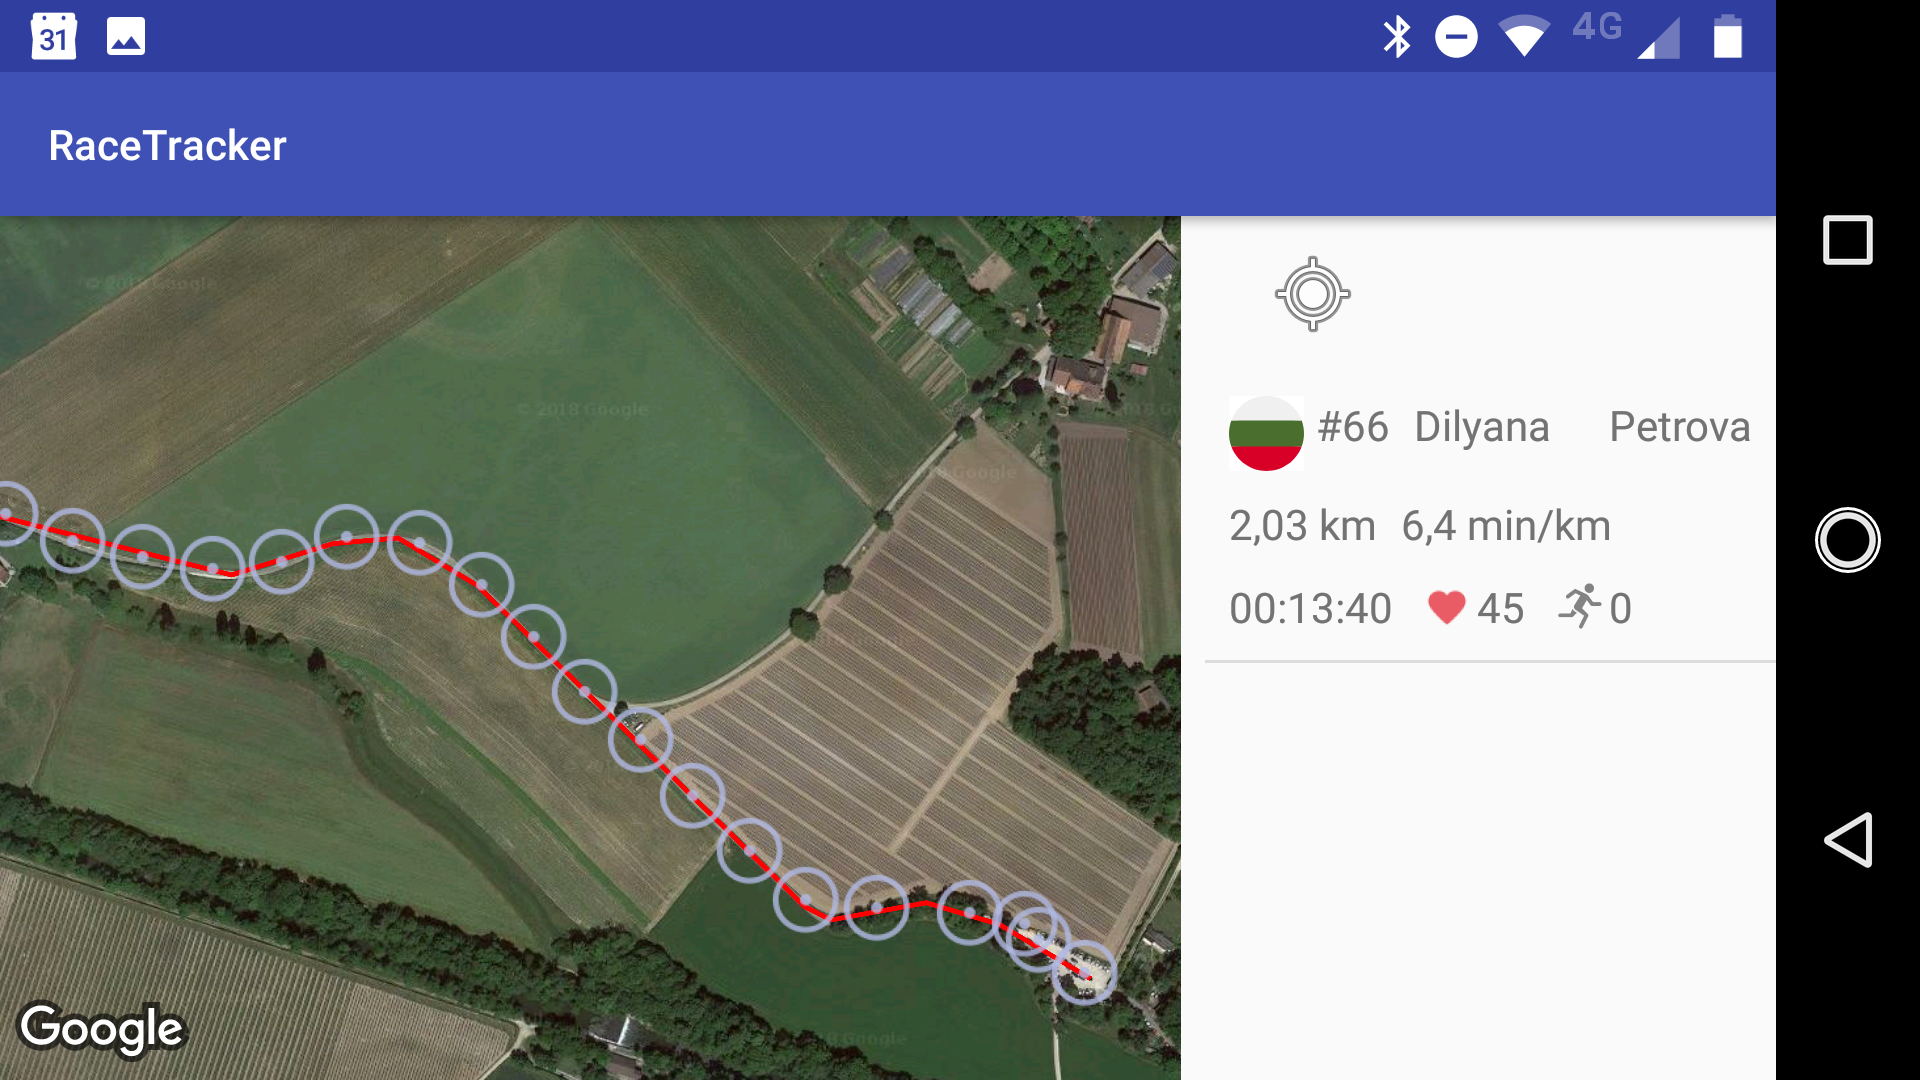
\includegraphics[width=0.9\linewidth]{test_distance_2_2.png}
  \caption{Test de distance \#2 - Image \#2}
  \label{fig:test_distance_2_2}
\end{subfigure}%

\begin{subfigure}{0.9\textwidth}
  \centering
  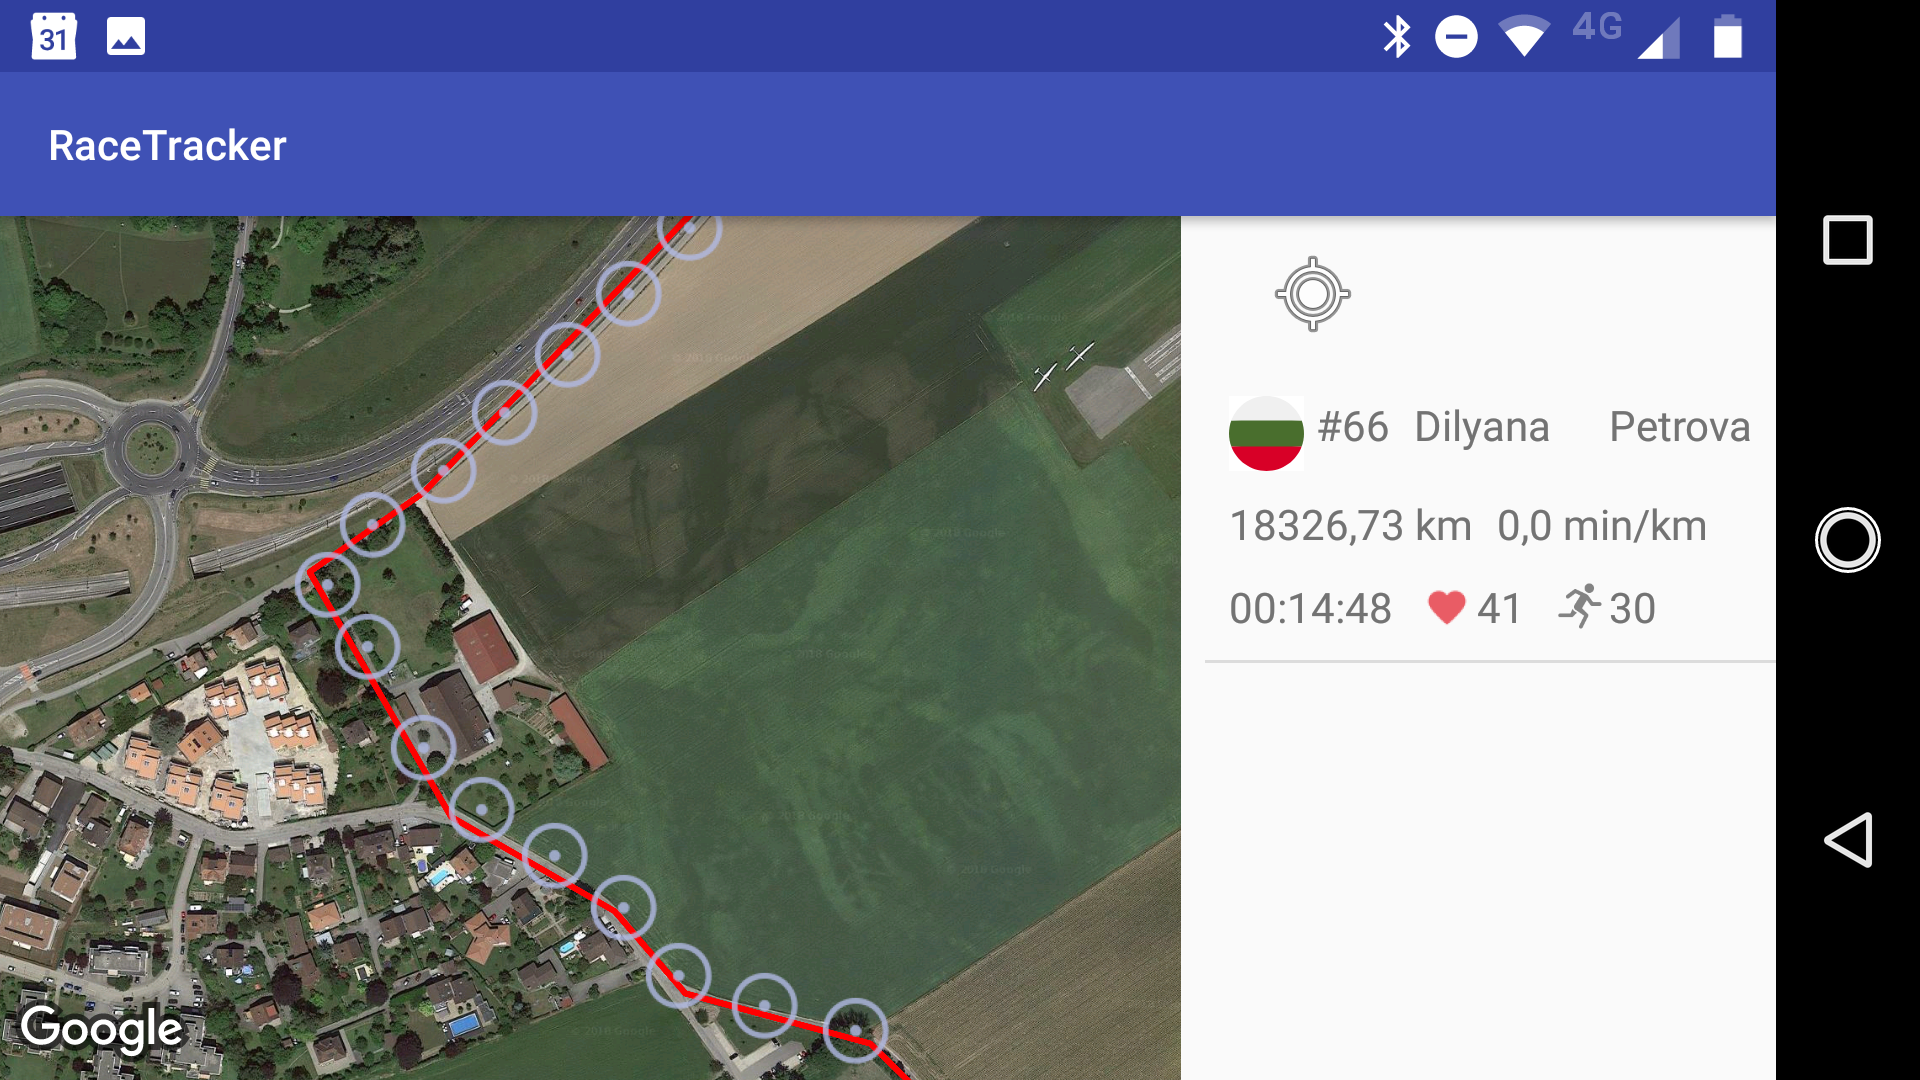
\includegraphics[width=0.9\linewidth]{test_distance_2_3.png}
  \caption{Test de distance \#2 - Image \#3}
  \label{fig:test_distance_2_3}
\end{subfigure}
\caption{Détail du parcours du test de distance \#2}
\label{fig:test_distance_2_2}
\end{figure}

\section{Test de durée}

Pour pouvoir déterminer combien de temps le capteur est capable de rester en fonction avec comme seule source d'énergie l'accumulateur, un test est effectué  où le capteur est programmé pour envoyer régulièrement des paquets de données à la passerelle exactement comme il le ferait pendant une course.

Le système est laissé comme cela le plus longtemps possible. On rappelle que le cahier des charges stipule que le capteur doit avoir une autonomie d'au moins 10 heures afin de pouvoir être utilisé pendant l'entièreté d'un événement.

Le test a démarré le Dimanche 23 Septembre 2018 à 20h10 et le capteur fonctionnait toujours le Lundi 24 Septembre à 16h00. A ce moment-là il a dû être débranché afin de pouvoir faire le test de distance. La durée totale de fonctionnement correspond donc à 19 heure 50 minutes, bien au-delà des 10 heures requises par le cahier des charges.

Il est nécessaire de préciser que cette durée peut être grandement influencée par la configuration du capteur. En effet, la puissance du signal LoRa émis durant l'envoi des paquets est directement corrélée avec la consommation d'énergie. Plus la puissance est élevée, plus la consommation sera haute. Si l’on se réfère à la data sheet du module LoRa RN2483, voir document \cite{rn2483-datasheet-real} p.8, on peut trouver la consommation en mA de chaque configuration de puissance. On notera que pour la configuration de base du module, c'est-à-dire -0.6 dBm, la consommation est de 21.2 mA. Avec une puissance du signal maximale de 14.1 dBm on peut voir que la consommation est pratiquement doublée à 38.9 mA. Il est donc nécessaire de prendre garde à la configuration que l'on utilise si l'on veut optimiser la durée de vie du capteur.